\section{Die Daten}\label{die daten}
Die Datengrundlage für die Netze werden von dem DWD in Form des Radar Online Aneichungs verfahren (RADOLAN) zur Verfügung gestellt. Das RADOLAN verfahren kombiniert die Messungen der 18 Radarstation und den punktuellen Messungen von über 2000 Bodenniederschlagsstationen (https://www.dwd.de/DE/leistungen/radolan/radolan.html). Eine dieser Bodenniederschlagsstationen befindet sich in Konstanz. 

\begin{figure}[htb]
 \centering
 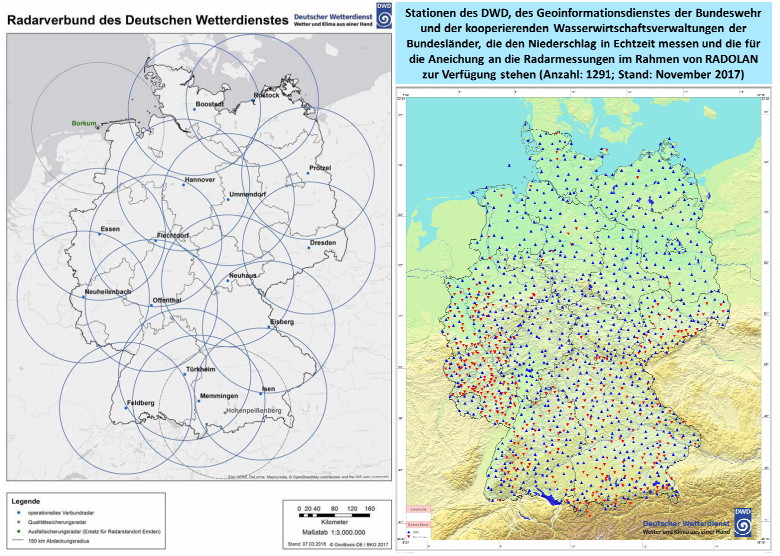
\includegraphics[width=0.6\textwidth,angle=0]{abb/daten_stationsuebersicht}
 \caption[Stationen Übersicht]{Übersicht über alle Boden und Radarstationen}
\label{fig:daten_stationsuebersicht}
\end{figure}

Um die Qualität der aus den RADAR Daten gewonnenen PNGs zu überprüfen, wurden die PNGs mit den Niederschlagsdaten von der Bodenstation in Konstanz verglichen. Die Daten der Station stehen in ein und zehn minütiger Auflösung zur Verfügung. Da sich herausstellte, dass bei der ein minütigen Auflösung Daten Fehlen, wurden die Daten der 10 minütigen Auflösung verwendet um die PNGs zu validieren. 
Die RADOLAN Daten für die Netze werden über den Opendata Server vom DWD zur Verfügung gestellt. Die Binärdaten werden je nach Jahr in Form eines 1100x900 oder 900x900 Pixel Gitter über Deutschland gelegt.  Dabei entspricht jeder Pixel 1km x 1km. Jeder Pixel in dem Pixel Koordinatensystem hat dabei zugehörige Höhen und Breitengrad Koordinaten. In folgender Abbildung ist der Aufbau der Binärdaten zu sehen.

\begin{figure}[h]
 \centering
 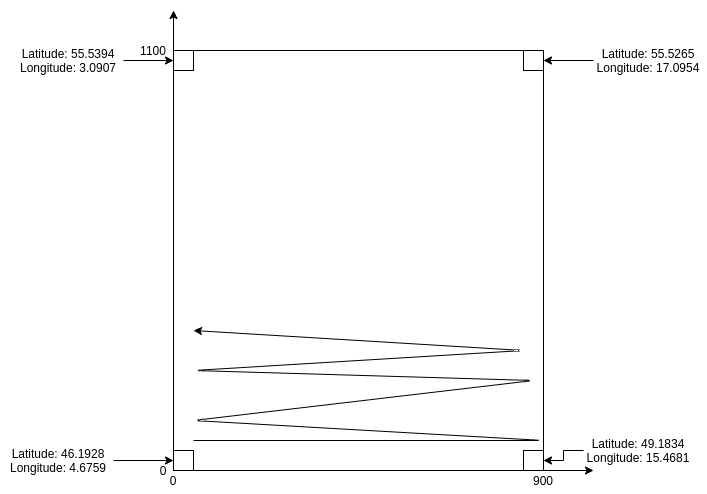
\includegraphics[width=0.8\textwidth,angle=0]{abb/radolan_koordinatensystem_aufbau}
 \caption[Aufbau des Koordinatensystems von Binärdaten]{Der Aufbau des Koordinatensystems der Radar Daten}
\label{fig:radolan_koordinatensystem_aufbau}
\end{figure}

Wie zu sehen ist, befinden sich der Pixel (0|0) in der Ecke unten links. Bei der Datenvorverarbeitung wird das Array mit den Pixeln jedoch von oben Links beginnend gefüllt, was bei dem entstehenden PNG  zu einer Spiegelung von 90 grad um die vertikale Achse führt (Siehe Kapitel Datenaufbereitung). 
Des weiteren ist zu beachten, dass die Breitengrade in den Ecken nicht übereinstimmen. So hat die Ecke unten Links einen größeren Breitengrad als die Ecke oben Links. Das gleiche ist auch bei den Höhengraden zu beobachten. Die Ursache hierfür ist die Transformation der Daten von einer 3D Kugel auf eine 2D Karte. In Abbildung \ref{fig:karte_abdeckung_daten} ist das daraus resultierende Ergebnis abgebildet. 

\begin{figure}[H]
 \centering
 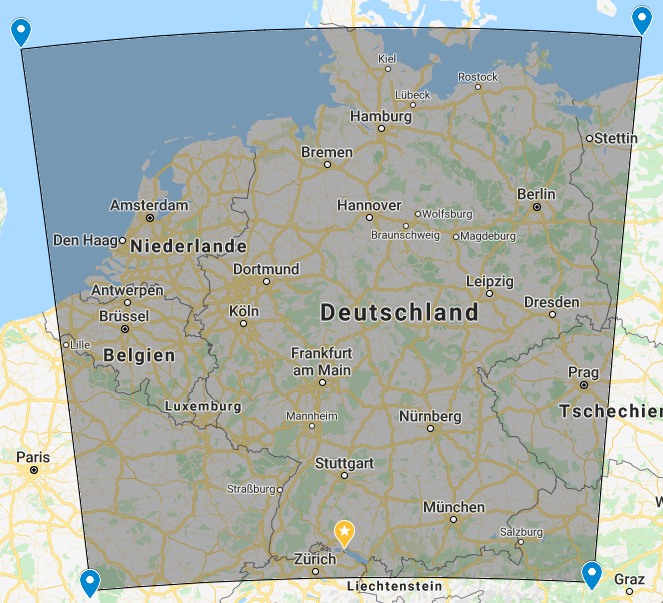
\includegraphics[width=0.6\textwidth,angle=0]{abb/karte_abdeckung_daten}
 \caption[Von Daten abgedeckte Fläche]{Die von den Daten abgedeckte Fläche auf einer 2D Karte}
\label{fig:karte_abdeckung_daten}
\end{figure}